\documentclass[letter,11pt,oneside]{article}
%%% HEREHEREHERE
%%% APPENDIX
%%% (insert (format "%s" (buffer-file-name)))
% /home/wayne/git/external/SAS_3DSpectrographs/tex/SpecroArticle.tex
%%% (occur "\\(\\\\[a-z]*section\\|appendix\\|input\\|\\<include\\>\\)")

%%\documentclass[11pt,twocolumn]{article}
%%\usepackage[inline]{asymptote}       %% Inline asymptote diagrams
%%\usepackage{wglatex}                 %% Use this one and kill others.
\usepackage{color}                     %% colored letters {\color{red}{{text}}
\usepackage{fancyhdr}                  %% headers/footers
%%\usepackage{fancyvrb}                %% headers/footers
\usepackage{datetime}                  %% pick up tex date time 
\usepackage{lastpage}                  %% support page of ...lastpage
\usepackage{times}                     %% native times roman fonts
\usepackage{textcomp}                  %% trademark
\usepackage{amssymb,amsmath}           %% greek alphabet
\usepackage{parskip}                   %% blank lines between paragraphs, no indent
\usepackage{shortvrb}                  %% short verb use for tables
\usepackage{lscape}                    %% landscape for tables.
\usepackage{longtable}                 %% permit tables to span pages wg-longtable
\usepackage{multicol}                  %% Enhance footnotes/endnotes
\usepackage{url}                       %% Make URLs uniform and links in PDFs
\usepackage{enumerate}                 %% Allow letters/decorations for enumerations
\usepackage{endnotes}                  %% Enhance footnotes/endnotes
\usepackage{listings}                  %% Make URLs uniform and links in PDFs
\pdfadjustspacing=1                    %% force LaTeX-like character spacing
\usepackage{geometry}                  %% allow margins to be relaxed
%%\usepackage{wrapfig}                 %% permit wrapping figures.
%%\usepackage{subfigure}               %% images side by side.
\geometry{margin=1in}                  %% Allow narrower margins etc.
\usepackage[T1]{fontenc}               %% Better Verbatim Font.
\renewcommand*\ttdefault{txtt}        %% 
\usepackage[colorlinks=true]{hyperref} %% Make huperlinks within a PDF
\usepackage{natbib}                    %% bibitems


%% include background image (wg-document-page-background) 

\usepackage{graphic
x}            %% Include pictures into a document
%% (wg-texdoc-inserttikz)

\usepackage{pgf,tikz,pgfplots}
\pgfplotsset{compat=1.15}
\usepackage{mathrsfs}

\usetikzlibrary{decorations.pathreplacing}
\usetikzlibrary{decorations.markings}
\usetikzlibrary{calc}
\usetikzlibrary{arrows}
\pgfplotsset{every tick label/.append style={font=\tiny}}


\newcommand{\degre}{\ensuremath{^\circ}}
\definecolor{qqwuqq}{rgb}{0,0.39215686274509803,0}
\definecolor{qqqqff}{rgb}{0,0,1}
\definecolor{uuuuuu}{rgb}{0.26666666666666666,0.26666666666666666,0.26666666666666666}
\definecolor{ududff}{rgb}{0.30196078431372547,0.30196078431372547,1}
\definecolor{ffqqqq}{rgb}{1,0,0}
\definecolor{xdxdff}{rgb}{0.49019607843137253,0.49019607843137253,1}


\def\documentisdraft{NOTDRAFT}

%% (wg-texdoc-isdraft)


\def\drafttest{DRAFT}
\def\wgdocdate{01 Aug, 2020}
\def\wgdocdatetime{\wgdocdate at \currenttime}
\ifx\documentisdraft\drafttest
\usepackage[left]{lineno}   %%%%%%%%%%%%% DRAFT
\usepackage{draftwatermark}
%%\SetWatermarkScale{5.0}
%%\SetWatermarkColor[gray]{0.3}
\fi

%% (wg-texdoc-insert-fancy-headers)

%%\usepackage[bookmarks]{hyperref} %% Make huperlinks within a PDF
%%\usepackage{makeidx}             %% Make an index uncomment following line
%%\makeindex                       %%.. yeah this one, too. index{key} in text
%%


\newcommand{\taninv}{Tan^{-1}}
\definecolor{verbcolor}{rgb}{0.6,0,0}
\definecolor{darkgreen}{rgb}{0,0.4,0}
\newcommand\debate[1]{\textcolor{darkgreen}{DEBATE: #1} \marginpar{\textcolor{red}{DEBATE} }}
\newcommand{\ltodo}[2]{\marginpar{\textcolor{red}{ACTION: #1}\endnote{#2}}}
\renewcommand{\thefigure}{\thesection-\arabic{figure}}
\newcommand{\menu}{\ensuremath{\;\rightarrow\;}}
\newcommand{\dhl}[1]{{\color{verbcolor}{\texttt#1}}}
\definecolor{wglightgreen}{rgb}{0.88, 0.58, 0.88}
\newcommand{\wgtextbox}[1]{\noindent\fcolorbox{darkgreen}{wglightgreen}{%
    \minipage[t]{\dimexpr0.80\linewidth-2\fboxsep-2\fboxrule\relax}
        {#1}
    \endminipage}}
%%(wg-add-inline-images)  %% add inline images to the mix





%%Begin User Definitions: Hint: ~/.latex.defs and  latex.defs  
%%End User Definitions:
%% (wg-texdoc-adjust-paper-width)
%% (wg-texdoc-insert-hypersetup)
%% (wg-latex-tablet-page)


%%%%%%%%%%%%%%%%%%%%%%%%%%%%%%%%%%%%%%%%%%%%%%%%%%%%%%%%%%%%%%%%%%%%%%%%%%%%%


\begin{document}


%% (wg-latex-pretty-title-page)
%% (wg-texdoc-titleblock)


\title{Letter:\\
Spectrographic Calibration\\
~ \\
{\large Flood vs Beam vs On Axis \\
Injection of Calibration References}}
\author{Wayne Green, Jerry Foote, Clarke Yeager, Anthony Rodda}
\date{\today}
\maketitle

\begin{abstract}
This letter reports preliminary results with spectrographic
calibration of small telescope spectrographs. We have experienced
thermal expansion and mechanical flexture. We are investigating using
a converging beam with the same f/ratio and PSF as a star. This is
proving hard to do. Recent discussions has brought us to consider the
problem from several aspects. These results mainly center on the
LOWSPEC family of spectrograph by Paul Gerlach.

\end{abstract}

%%%%%%%%%%%%%%%%%%%%%%%%%%%%%%%%%%%%%%%%%%%%%%%%%%%%%%%%%%%%%%%%%%%%%%%%%%%%%
%% table of contents
%%%%%%%%%%%%%%%%%%%%%%%%%%%%%%%%%%%%%%%%%%%%%%%%%%%%%%%%%%%%%%%%%%%%%%%%%%%%%
 
\pagenumbering{roman}   % i,ii,etc
%%\pagenumbering{gobble}   %ignore page numbers for a while
\pdfbookmark[0]{Table of Contents}{MyTOC} % if usepackage{hyperref} in use.
\tableofcontents
%\listoffigures
\listoftables
\newpage


\setcounter{section}{0}
\pagenumbering{arabic}

\ifx\documentisdraft\drafttest
\linenumbers    %%%%%%%%%%%%% DRAFT
\fi

\section{Overview}

For about 18 months the cohort suffered Green saying to ignore the
signal and focus on the noise. If noise is kept under acceptable
control -- the science result's signal can be shown to be
objectively better. 

One critical source of ``noise'' is calibration line shift, accuracy,
usefulness in the recent Spectro-L thread.

The short question is between utilizing a gas lamp for reference
calibration lines by flooding a slit (flood) or using a precisely
formed converging beam (beam). The Question come down to the quality
of lines made by the lamp, and how does the impact of a simple
experiment of subtracting the first comp image from the last comp
image -- assuming one has followed a strategy along the lines of 1)
comp-sci-sci-sci-comp or 2) comp-sci-comp-sci-comp-sci-comp. Flats
have important questions of their own but are not germane to this
question.



IRAFs answer to how to subtract images comp1.fits from comp2.fits:
\dhl{imarith comp1 - comp2 diff.fits}. We've seen shifts of several
pixels across one observation.


Answering the difference between flood vs beam,. first start with
the ``thin lens equation''\footnote{The ``lens makers formula'' deals with
the radius of curvature for lens surfaces. Appendix \ref{sec:lensmakersformula}.}:

\begin{figure}[h!]
\centering
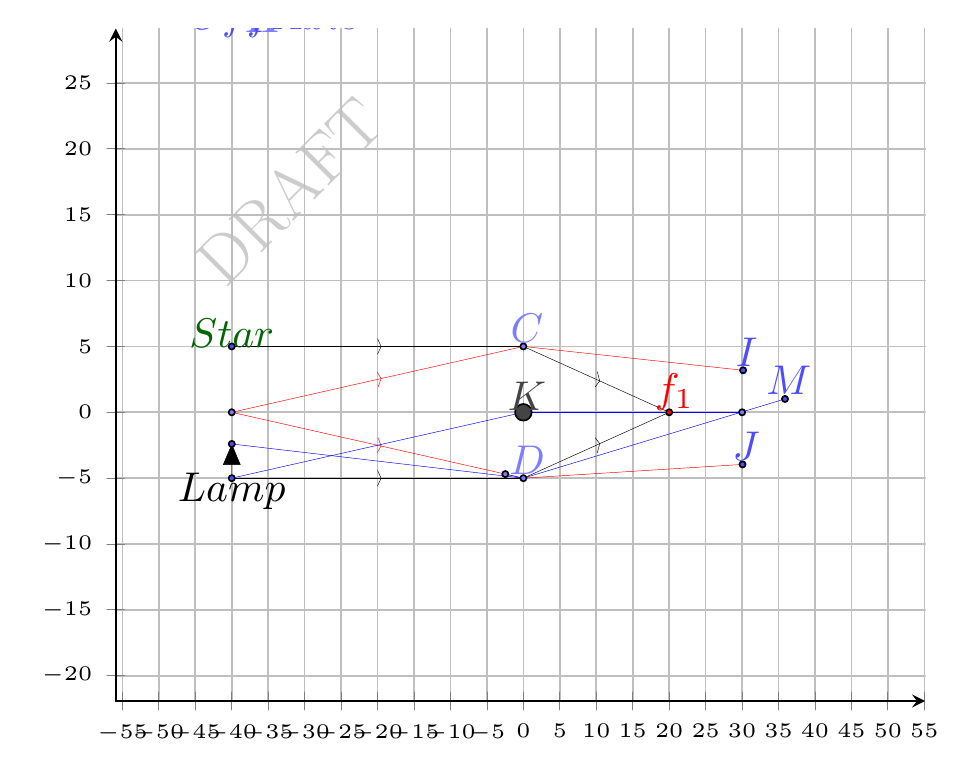
\begin{tikzpicture}[line cap=round,line join=round,>=triangle 45,scale=1.5]
\begin{axis}[
%x=1cm,y=1cm,
%axis lines=middle,
separate axis lines, % important !
axis x line=bottom,
axis y line=left,
ymajorgrids=true,
xmajorgrids=true,
xmin=-55.908428957138916,
xmax=55.117646309668594,
ymin=-21.91544157915341,
ymax=29.136905260878166,
xtick={-55,-50,...,55},
ytick={-20,-15,...,25},
]
\clip(-55.908428957138916,-21.91544157915341) rectangle (55.117646309668594,29.136905260878166);
\draw [shift={(20,0)},line width=0.11pt,color=qqwuqq,fill=qqwuqq,fill opacity=0.10000000149011612] (0,0) -- (165.96375653207352:1.9436172654834343) arc (165.96375653207352:194.03624346792648:1.9436172654834343) -- cycle;
\draw [shift={(20,0)},line width=0.11pt]  plot[domain=2.896613990462929:3.3865713167166573,variable=\t]({1*20.615528128088304*cos(\t r)+0*20.615528128088304*sin(\t r)},{0*20.615528128088304*cos(\t r)+1*20.615528128088304*sin(\t r)});
\draw [shift={(-20,0)},line width=0.11pt]  plot[domain=-0.24497866312686423:0.24497866312686414,variable=\t]({1*20.615528128088304*cos(\t r)+0*20.615528128088304*sin(\t r)},{0*20.615528128088304*cos(\t r)+1*20.615528128088304*sin(\t r)});
\draw [line width=0.11pt] (-40,5)-- (0,5);
\draw [line width=0.11pt] (-19.514095683629144,5) -- (-20,4.416914820354969);
\draw [line width=0.11pt] (-19.514095683629144,5) -- (-20,5.583085179645031);
\draw [line width=0.11pt] (-40,-5)-- (0,-5);
\draw [line width=0.11pt] (-19.514095683629144,-5) -- (-20,-5.583085179645027);
\draw [line width=0.11pt] (-19.514095683629144,-5) -- (-20,-4.4169148203549655);
\draw [line width=0.11pt] (0,5)-- (20,0);
\draw [line width=0.11pt] (10.471396428315431,2.3821508929211404) -- (9.858581071505368,1.934324286021478);
\draw [line width=0.11pt] (10.471396428315431,2.3821508929211404) -- (10.141418928494627,3.0656757139785182);
\draw [line width=0.11pt] (0,-5)-- (20,0);
\draw [line width=0.11pt] (10.471396428315431,-2.3821508929211404) -- (10.141418928494627,-3.0656757139785182);
\draw [line width=0.11pt] (10.471396428315431,-2.3821508929211404) -- (9.858581071505368,-1.934324286021478);
\draw [line width=0.11pt,color=ffqqqq] (-40,0)-- (0,5);
\draw [line width=0.11pt,color=ffqqqq] (-19.51784789666552,2.560269012916807) -- (-19.92767718449983,1.9214174759986171);
\draw [line width=0.11pt,color=ffqqqq] (-19.51784789666552,2.560269012916807) -- (-20.072322815500176,3.0785825240013756);
\draw [line width=0.11pt,color=ffqqqq] (0,5)-- (30.13641626049038,3.1885778314936446);
\draw [line width=0.11pt,color=ffqqqq] (-40,0)-- (0,-5);
\draw [line width=0.11pt,color=ffqqqq] (-19.51784789666552,-2.560269012916807) -- (-20.072322815500176,-3.0785825240013756);
\draw [line width=0.11pt,color=ffqqqq] (-19.51784789666552,-2.560269012916807) -- (-19.92767718449983,-1.9214174759986171);
\draw [line width=0.11pt,color=ffqqqq] (0,-5)-- (30.05875237342711,-3.956499778327017);
\draw [->,line width=0.11pt] (-40,-5) -- (-39.994073757640564,-2.4032220370616653);
\draw [line width=0.11pt,color=qqqqff] (-40,-5)-- (0,0);
\draw [line width=0.11pt,color=qqqqff] (0,0)-- (30,0);
\draw [line width=0.11pt,color=qqqqff] (35.8835439031722,1.0139889937221238)-- (0,-5);
\draw [line width=0.11pt,color=qqqqff] (0,-5)-- (-2.477069759962774,-4.690366280004653);
\draw [line width=0.11pt
,color=qqqqff] (-39.994073757640564,-2.4032220370616653)-- (0,-5);
\begin{scriptsize} % scriptsize
\draw [fill=xdxdff] (130.40312238249933,0) circle (0.75pt);
\draw[color=xdxdff] (-35.64927998840779,29.88195854598015) node {$A$};
\draw [fill=ffqqqq] (20,0) circle (0.75pt);
\draw[color=ffqqqq] (20.71562071061181,1.5699337121047707) node {$f_{1}$};
\draw [fill=xdxdff] (0,5) circle (0.75pt);
\draw[color=xdxdff] (0.5020011495840906,6.364189633630578) node {$C$};
\draw [fill=xdxdff] (0,-5) circle (0.75pt);
\draw[color=xdxdff] (0.5020011495840906,-3.6130456625177243) node {$D$};
\draw [fill=ududff] (-40,5) circle (0.75pt);
\draw[color=ududff] (-35.64927998840779,29.88195854598015) node {$F$};
\draw [fill=ududff] (-40,-5) circle (0.75pt);
\draw [fill=xdxdff] (-40,0) circle (0.75pt);
\draw[color=xdxdff] (-35.64927998840779,29.88195854598015) node {$H$};
\draw [fill=ududff] (30.13641626049038,3.1885778314936446) circle (0.75pt);
\draw[color=ududff] (30.628068764577325,4.550146852512706) node {$I$};
\draw [fill=ududff] (30.05875237342711,-3.956499778327017) circle (0.75pt);
\draw[color=ududff] (30.563281522394544,-2.576449787593225) node {$J$};
\draw [fill=ududff] (-39.994073757640564,-2.4032220370616653) circle (0.75pt);
\draw[color=ududff] (-34.09438617602105,29.88195854598015) node {$OffAxis$};
\draw [fill=uuuuuu] (0,0) circle (2pt);
\draw[color=uuuuuu] (0.5020011495840906,1.2459975011908648) node {$K$};
\draw [fill=xdxdff] (30,0) circle (0.75pt);
%\draw[color=xdxdff] (30.498494280211762,1.375571985556427) node {$L$};
\draw [fill=ududff] (35.8835439031722,1.0139889937221238) circle (0.75pt);
\draw[color=ududff] (36.394133318844844,2.4121678604809262) node {$M$};
\draw [fill=xdxdff] (-2.477069759962774,-4.690366280004653) circle (0.75pt);
%\draw[color=xdxdff] (-1.959914053361593,-3.2891094516038186) node {$N$};
%\draw[color=qqwuqq] (22.52966349172968,6.46855059499749047) node {$\theta = 28.07\textrm{\degrees}$};
\draw[color=qqwuqq] (-40,6) node {$Star$};
\draw[color=black] (-40,-6) node {$Lamp$};
%\draw (-5cm,0) arc[radius = 5cm, start angle = 355, end angle = 5] ;
\end{scriptsize} % scriptsize
\end{axis}
\end{tikzpicture}

\caption{Lens Makers Formula with star and cal-lamp light. (Not happy
with the rendering -- Tikz needs upgrading.)}
\label{fig:LMF}
\end{figure}


\begin{align}
\frac{1}{f} &= \frac{1}{s_{1}} +  \frac{1}{s_{2}} 
\end{align}

where f is the actual focal length of the lens/lens assembly for
infinity ; $s_{1}$ is the
distance from the lens to the target and $s_{2}$ is the distance from
the lens to the virtual image.


A few waypoints to
notice: if $s_{1}$ is essentially at infinity, then $\frac{1}{s_{1}}$
goes to zero and the position $s_{2}$ is equal to the stated focal
length. The next very interesting thing is that if a light is placed
at $s_{2}$ (L--D not shown), the beam is essentially parallel -- or at
infinity and is said to be collimated.

In Fig. \ref{fig:LMF} there should be a lens indicated along C--K--D
that did not render.  In the spectrograph, the slit is at $f_{1}$.
The arrow is an off-axis near-field bulb filiment, producing a ray
Lamp\menu D \menu M, where the star's ray, along the same path, is
from infinity \menu D \menu ${f_{1}}$. The two angles are not the
same. Taking a bundle of lines along the filiment of the lamp produces
a series of rays -- each with a different angle. Variation in the
position of the lamp can cause a mis-match of calibration
locations. There is also a bias from the position of the bulb
w.r.t. the slit.

If $s_{1}$ is close to the lens, then the rays are diverging into the
lens and come to focus at $s_{2}$ some distance farther out than the
focal length of the lens. The angle of the rays fall within the
range subtended by the geometry of the circle or rays hitting the lens
surface. A wider range, the closer the source to the lens. 

A critical thing to remember, is that the target itself (size of the
bulb -- say the two electrodes) causes a mix of angles of rays in the
bulb's beam. This adds up to more variance in incidence angles at the
grating.

Flooding has diverging beams, acts like a ``near-field'' target and
therefore the focus of the collimator is wrong w.r.t. a grating. By
the grating equation, this generates a diverging beam at the grating
-- the incidence angle of rays at the 'right' side will be different
than those from the 'left' side. This in essence effects the focus.
Flooding off axis produces an asymmetry in the output of the
collimator and will produce a ``corresponding'' shift in the lens. The
asymmetry is introduced by changes due to thermal expansion and with
flexure.  Focusing with the comp lamp is invalid. Focusing with sky
lines late in afternoon is much better.

For reference, the grating equation for a reflection grating:


\begin{align}
\frac{m\lambda}{d} &= sin(\alpha) + sin(\beta)
\end{align}

where $m$ is the mode, $\lambda$ in wavelength, $\alpha$ is the
``angle if incidence'' and $\beta$ is the ``angle of diffrection''.
The near-field lamp produces a wide range of $\alpha$ incidence angles
that are not consistent with the far-field stellar image. The addition
operator needs to be subtraction for transmission gratings.

\textbf{\emph{Summary 1:}} Co-linear rays from the collimator to the grating improves
the overall placement, line shape, and line width (focus) of the resulting
spectra. Repeatable variations will produce a systematic wavelength
identification. Non-repeatable variations due to variations in temperature
and flexure introduce random wavelength positions.

\subsection{Mitigation Strategies}

Use a diffusing screen. This converts more coherent (not very coherent
to begin with straight from the bulb) into a ``Lambertian'' source.
The Lambertian source is usually depicted with a single point and 
speaks to the intensity at different angles projected away from that point.
Integrating over all points boils down to a large mix of rays at different
angles.

\textbf{\emph{Summary 2:}} One can argue the narrow width of the slit mitigates the
use of a flooding lamp, but measurements shows a small shift -- one
that can amount to 10s to 1000s of km s-1 in the spectra.

\textbf{\emph{Summary 3:}} With energy  $E=h\nu$ relates to wavelength ($lambda$)
as $\nu = c/\lambda$, a shift in wavelength improperly converted
to the targets frame of reference amounts to a misstatement of
Energy. This is not accounted for through the line ratio analysis
process.

\textbf{\emph{Summary 4:}} It is obvious that radial velocity statements mis-stated
as the $\Delta{\lambda}$ is non-linear and a shift due to mis-identification
will have a material impact on radial velocity statements.

Mitigation by solving a spectrum using sky-lines or using the absorption
features in the target itself (within the targets frame of reference)
will help with line ratios. Solving with both sky-lines and with
the target gives the shift needed to state the radial velocity.

\subsection{Beam Case}

Great idea, difficult to implement. The general idea is a diffusion
method (scattering screen, microlenses, integrating sphere), a 
collimator, a matching f/ratio lens for the star's image and
a way to match the injection angles. Its the injection matching
that is proving mechanically difficult.

\section{Conclusion}

The use of comp lamps may be done away with if sufficient information
in the form of sky-lines (light pollution and tellurics). Nodding
the telescope and employing a sufficient exposure time can solve
the flood vs beam question. In may cases, small telescope spectroscopy
is well suited to detect and report gross changes of state with 
a target, and to help qualify novae. Novae respond well to low
SNR and to very low R values. We have ignored many issues in this
discussion that bear thought.


\appendix
\renewcommand \thesection{\Alph{section}}

\section{Science Objectives}


The quintessential aspects of spectral reduction boils down to the
energy physics represented by effective feature width or the centroid
of a target's features for radial velocity study. Small telescope
spectrographs are in the R$\sim$ 600,1000,10000 range, generically
for the Alpy, Lisa and LHires/echelle products from Shelyak.
The prominent features include H$\alpha$ or nova lines. R is
essentially $\Delta{\lambda}/\lambda$, and for H$\alpha$ of
say 6000\AA\; then the Alpy should have a 10\AA\; resolution.


\begin{align}
R &= \frac{\lambda}{\Delta{\lambda}} \\
\frac{\Delta{\lambda}}{\lambda} &= \frac{\Delta{\nu}}{\nu} = \frac{v}{c} \\
v &= \frac{c}{R}
\end{align}

Here, a gross simplification using H$\alpha$ as 6000\AA\;, 

\begin{table}[h!]
%\phantomsection
%\addcontentsline{toc}{section}{ TOC CAPTION}
% \setlength{\belowcaptionskip}{6pt} % adjust space under caption abovecaptionskip
% \renewcommand{\arraystretch}{1.3} % adjust line spacing
%\small{
%\begin{minipage}{\textwidth}     % for footnotes in table.
%\caption[TOC]{Gross Velocity in terms of Resolution R.}
\centering
\begin{tabular}{| r | r |}
%\MakeShortVerb{\|}
%\multicolumn{n}{fmt}{text for merged cols}
\hline
R      & v ( km s-1)    \\ 
\hline
600    & 500    \\ 
1000   & 300    \\ 
10000  & 29    \\ 
%% ones-based: \cline{a-b}
\hline
%%\DeleteShortVerb{|}
\end{tabular}
%%\end{minipage}    %% for footnotes  r@{.}l 
\caption{Gross Velocity in terms of Resolution R}
\label{table:GrossVelocityintermsofResolutionR}
%%} % end small etc
\end{table}

% (iv (setq tmp (mapcar (lambda (a) (/ constant-c a 1e5)) '(600.0 1000.0 10000.0) )))
%    (499.65409666666665 299.792458 29.9792458)


The spectrograph consists of essentially three parts: 1) the
telescope,  2) the slit and 3) the spectrograph's optics.

The slit samples the ``focal plane'' from the telescope, a virtual
image, at point of focus.  The focus in the point of convergence for a
bundle of rays from a science target (star, chunk of nebula, sky
etc). The ray bundle is described well enough by the f/ratio of the
main telescope. Oversimplifying, it is a consistent converging bundle
of rays.

Other aspects that are often ignored include coma (off-axis aspect of
where the slit position falls w.r.t.  the telescope's curved focal
plane) and other attendant astigmatisms. The so called focal ``plane''
is actually curved -- unless flattened by additional optics. See
\citep{1898AJ.....19...17S} for mind numbing details. A flat plane is
common with Ritchey-Crit\'erion telescopes and to a high degree with
the CDK telescopes. Refractors, prone to field curvature will have
Petzval correctors, or may use other flatteners. Newtonians may use a
``Paracor'' \texttrademark or other optics. Longer focal lengths
suffer less but carry larger spot sizes for stars.

Also note the date of Schaeberle's publication. Schaeberle's concerns
center on the fact that most casual thought centers on the principle
ray along the optical axis.

The shape of this focal plane, and the field's energy contribution to
each point on the focal plane surface is way to complicated to delve
into here. The simplifying assumption is that the slit is tiny w.r.t.
the surface; the desired image is tightly defined by the f/ratio's
converging beam and aberrations can be ignored within an appropriate
over-simplifying assumption. Assumption about 'out of focus' rays
often miss the fact that the rays do not have the same f/ratio as the
desired science image and that those contributions (mainly sky in the
general case here) are axi-symmetric. They fail to become collimated,
and present focus and shift issues for use with spectral calibration.


The injection of the cal and flat lamps do not necessarily
satisfy these conditions. The main problem appears to be the
issue of rays from the cal lamp are off-axis, non axi-symmetric,
do not collimate in the same fashion as the science image
and therefore present a range of angles of incidence at the
grating. This in turn presents a range (both focus and shift)
in the lines at the camera's sensor. We have measured this
effect with simple experiments with the LOWSPEC spectrograph.

Our main issue with the LOWSPEC is flexure and thermal expansion.
To minimize these issues we are currently re-conducting the
experiment in a more temperature controlled setting using
stiff aluminum breadboards to host the LOWSPEC 3D printed
optics.

Most SCTs are a train-wreck of design trade-offs. Richard Berry
did a white paper that shows the best optical performance is
only about 125mm behind the telescope. This distance is quite
short. This means inserting guiders is a bit of bother.


A key problem of mismatching the f/ratio of the incoming beam w.r.t.
to a spectrograph's collimating lens/mirror is the slit is now
out of focus, and producing a range of angles of incidence
to the grating. The focus mismatch has the effect of skewing
these angles w.r.t. the position of the slit and optical axis.

The answer, for LOWSPEC, is to provide a prescription for the
collimating lens and to accommodate the lens. The distance
from the collimator to the grating is flexible -- the distance
to the slit is not. 



\section{The lens makers' formula (for completeness)} \label{sec:lensmakersformula}

\begin{subequations}
\begin{align}
P_{\tt{lens}} &= \frac{n_{\tt{lens}} - n_{0}}{n_{o}} \left( \frac{1}{R_{1}} - \frac{1}{R_{2}} \right) \\
\Phi{\lambda} &= \exp\left(\frac{2\pi i}{\lambda} \frac{r^2}{2f}\right) & \tt{phase} \label{eq:hob}
\end{align}
\end{subequations}

where $P_{\tt{lens}}$ is the ``Power'' in diopters, $n$ is the index
of refraction, $R_{1}$ is the radius of the ``front'' of the lens and
$R_{2}$ is the radius of the ``back'' of the lens. Equation
\eqref{eq:hob} wrecks merry-hob in terms of chromatic aberration --
another name for different wavelengths of light coming to focus at
different points, or with different angles of incidence.


\section{Magnitude Drop with Beam Splitter}

There is a commercial spectrograph that uses a beam splitter. Assuming
a 90\% transmission a 10\% loss amounts to 0.114.


\begin{align}
\Delta\:{\tt{mag}} &= -2.5 \frac{\Delta{I}}{1} \\
    0.114\; \tt{mag} &= -2.5 \times log_{10}(.90)
\end{align}

Along the beamsplitter's 10\% axis, injecting a conforming beam gives more
control over the exposure time and better photon statistics. 

% (iv (setq tmp (* -2.5 (log10 .90) )))   0.114

%%% ADDAPPENDIX


%% use a bibitem approach to the references publications etc.
%% (wg-bibitem)

%%\clearpage
\addcontentsline{toc}{section}{References}
\renewcommand*{\refname}{References}
\bibliographystyle{plain}	% bibliographystyle{apalike} and \usepackage{natbib}
\bibliography{SpecroArticle}{}	% expects file "MasterBib.bib"



%%\begin{thebibliography}{80}
%%\usepackage{natbib}   %% bibitems
%%\end{thebibliography}

%%\clearpage
%%\addcontentsline{toc}{section}{Index}
%%\printindex %% www.cs.usask.ca/resources/tutorials/latex/notes/toc-index.pdf

% /home/wayne/git/external/SAS_3DSpectrographs/tex/SpecroArticle.tex

%% (wg-texdoc-endnotes)
\end{document}

-----------------------------------------------------------------------------



Lets consider a optical setup where the $(X,Y)$ plane is along
the objective surface plane and $Z$ axis is the optical axis.
Lets assume axi-symmetric optics and ignore the $X$ axis.
So a piece of paper carrying a diagram consists of $Z$ in
the left-right direction and $Y$ in the up-down direction.


The telescope forms an image that is not necessarily along the optical
$Z$ axis. Best case, the optical axis is part of a perfectly aligned
telescope with a symmetrical Point Spread Function (PSF).  Coma is
introduced for stars off axis -- considered here to be some offset
above or below the $Z$ axis. Now consider the coma as being an
asymmetric beam passing into a slit location off-axis from the main
axis. Lets ignore all astigmatisms other than the coma.


The incoming beam from the telescope is at some f/ratio that is

\begin{align}
\tt{f/ratio} &= \frac{D}{fl} \\
\theta &= \taninv\frac{D}{fl}
\end{align}

My point comes with reconciling the incoming angles of incidence
w.r.t. the grating equation at the grating with the light from
the slit passing through the collimating lens. Up until now,
I have been discounting the significance of matching the f/ratio
of the collimating lens to the PDF of the telescope. 

Discussions with Bob Buchheim, SAS, has brought the FITS multispec
format to his attention, A Multispec file (several different bands of
equispec data) carries noise together with the spectrum each with its
own NAXIS. Discussions with Forrest Sims and Buchheim brought the
utility of storing image data for the reduced science image, the
calibration (comp) image and a sky band in a FITS
Multi-Extension-Format (MEF) format. I have been using both for years,
even bolting MEF into PyRAF with a few lines of Python for my personal
startup code. I have been promoting publishing properly flux
calibrated images using the multispec format.

